
\chapter{探索アルゴリズム}
\label{chap:basic-algorithm}
本章では,第\ref{chap:generalized-moore-graph}章で示した一般化ムーアグラフの
性質を利用して,与えられた頂点数と次数の一般化ムーアグラフを探索する基本的な
アルゴリズムを与える.これは後の章で探索空間を縮小する手法の比較対象となる.
まず,探索の初期状態と状態空間について説明した後,状態から新たな状態を生む
オペレータについて説明する.最後に,全体的なアルゴリズムを与える.

はじめに,次のムーアバウンドを定義する.
\begin{definition}\rm
  \textbf{ムーアバウンド}(\textbf{Moore bound})とは,
  次数が$k$,直径が$D$の正則グラフの頂点数の上界で,次式で定義される.
  \begin{equation}
    n_{k,D} = 1 + \sum_{i=1}^Dk(k-1)^{i-1}
  \end{equation}
\end{definition}
これは,同一の次数で$R=0$,$Q=D$の一般化ムーアグラフの頂点数に等しい.
ムーアバウンドを用いて探索の初期状態となる\textbf{初期グラフ}を定義する.
特に,定義\ref{def:basic-initial-graph}の初期グラフを\textbf{基本初期グラフ}と呼ぶ.
\begin{definition}\rm
  \label{def:basic-initial-graph}
  基本初期グラフとは,次のグラフ$G_I$である.
  \begin{equation}
    \begin{aligned}
      \label{eq:basic-initial-graph}
      G_I&=(V,E) \\
      V&=\{1,\ldots,n\} \\
      E&=\{(1,2),\ldots,(1,k+1)\}\cup
      \{(\text{parent}(v),v)|v=k+2,\ldots,n-R\} \\
      \text{parent}(v)&=
      \left\lceil\frac{v-n_{k,\hat{Q}(v)-1}}{k-1}\right\rceil+n_{k,\hat{Q}(v)-2}
    \end{aligned}
  \end{equation}
\end{definition}
基本初期グラフの例を図\ref{fig:initial-tree-example}に示す.

次に,探索空間の基底となる辺の列である\textbf{候補辺}を定義する.
\begin{definition}\rm
  \label{def:candidate-edges}
  候補辺$\{e_i\}_{i\in\mathbb{N}}$とは,初期グラフ$G_I$に対して,
  $G_I$上で次数が$k$未満の頂点同士を隣接させる辺のうち,$G_I$に属していない
  辺の集合に順序を付加した列である.具体的には,次の式で定義される.
  \begin{equation}
    \{e_i\}_{i\in\mathbb{N}} =
    \{(v,w)\,|\,d_{G_I}(v)<k,d_{G_I}(w)<k,(v,w)\in[V]^2\}\setminus E(G_I)
  \end{equation}
  便宜上,候補辺に属する辺も候補辺と呼ぶことにする.
\end{definition}
候補辺の定義より,一般化ムーアグラフの探索の探索空間は,候補辺から任意の個数の
辺を取り出した組合せと言える.
候補辺の例を図\ref{fig:feasible-edges-example}に破線で示す.

\begin{figure}
  \centering
  \begin{minipage}{.45\columnwidth}
    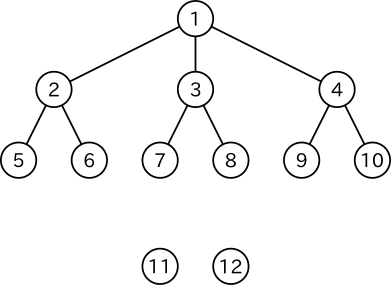
\includegraphics[width=\textwidth]{initial-tree-example.pdf}
    \captionof{figure}{基本初期グラフの例}
    \label{fig:initial-tree-example}
  \end{minipage}
  \hfill
  \begin{minipage}{.45\columnwidth}
    \def\svgwidth{\textwidth}
    \input{feasible-edges-example.pdf_tex}
    \captionof{figure}{候補辺の例(破線部分)}
    \label{fig:feasible-edges-example}
  \end{minipage}
\end{figure}

探索に用いる状態として,グラフ$G$と次に追加する候補辺の番号$i$の組を使う.
初期状態は,$(G_I,1)$である.状態$(G,i)$が与えられたとき,
候補辺$e_i$を追加するオペレータ(\textbf{追加オペレータ})と
追加しないオペレータ(\textbf{無追加オペレータ})の動作を与える.
追加オペレータは,与えられた状態$(G,i)$に対して,状態$(G+e_i,i+1)$を返す.
また,無追加オペレータは,与えられた状態$(G,i)$に対して,状態$(G,i+1)$を返す.

オペレータが適応可能な状態の条件を示す.その前に,次の記号を定義する.
\begin{definition}\rm
  頂点$v$と候補辺$\{e_i\}_{i\in\mathbb{N}}$について,$v$と接続している辺
  $e_i$の番号$i$の最小値と最大値をそれぞれ$\text{Enter}(v)$と
  $\text{Exit}(v)$とする.
  $\text{Enter}(v)$と$\text{Exit}(v)$の具体的な式は,次で与えられる.
  \begin{equation}
    \label{eq:frontier}
    \begin{aligned}
    \text{Enter}(v) &= \min\{i\,|\,v\in e_i\} \\
    \text{Exit}(v) &= \max\{i\,|\,v\in e_i\}
    \end{aligned}
  \end{equation}
\end{definition}

二種類のオペレータそれぞれについて,対象の辺以降の辺の選び方で
一般化ムーアグラフとなる見込みがあるかどうかを判定する方法を,
定理\ref{thm:gmg-geometric-property}より与える.
\begin{corollary-without-proof}\rm
  \label{coll:basic-add-operator}
  追加オペレータについて,与えられたグラフを$G$,候補辺番号を$i$,候補辺を
  $e_i=\{v,w\}$,適応後のグラフを$G'$とする.$i$以降の候補辺の
  選び方次第で$G'$が一般化ムーアグラフとなる見込み
  があることとは,次の二条件の両方を満たすことである.
  \begin{enumerate}
  \item 次数条件$\cdots$ $d_G(v)<k$かつ,$d_G(w)<k$かつ,
    $\text{Exit}(x)=i$なる$x\in e_i$について$d_{G'}(x)=k$
  \item 閉路条件$\cdots$ $d_G(v,w)\geq2Q$\\
    (この条件を満たすとき,$e_i$によってできる閉路の長さは少なくとも
    $2Q+1$となり,定理\ref{thm:gmg-geometric-property}を満たす)
  \end{enumerate}
\end{corollary-without-proof}
\begin{corollary-without-proof}\rm
  \label{coll:basic-noadd-operator}
  無追加オペレータについて,与えられたグラフを$G$,候補辺番号を$i$,候補辺を
  $e_i=\{v,w\}$,適応後のグラフを$G'$とする.$i$以降の候補辺の
  選び方次第で$G'$が一般化ムーアグラフとなる見込み
  があることとは,次の二条件の両方を満たすことである.
  \begin{enumerate}
  \item 次数条件$\cdots$ $\text{Exit}(x)=i$なる$x\in e_i$について,$d_{G'}(x)=k$
  \end{enumerate}
\end{corollary-without-proof}

最後に,説明した事柄を用いて深さ優先探索を一般化ムーアグラフの探索に適応する.
その手順をアルゴリズム\ref{algo:basic-algorithm}に示す.
\begin{algorithm}[H]
  \caption{一般化ムーアグラフの探索アルゴリズム}
  \label{algo:basic-algorithm}
  \begin{algorithmic}[1]
    \Require $n,k$
    \Ensure $M(n,k)\:$(見つからない場合,$\varnothing$を返す)
    \Procedure{FindGeneralizedMooreGraph}{}
    \State $G_I\gets\text{初期グラフ}$
    \Comment 定義\ref{def:basic-initial-graph}
    \State $\{e_i\}_{i\in\mathbb{N}}^M\gets G_I\text{の候補辺}$
    \Comment 定義\ref{def:candidate-edges}
    \State $Stack\gets((G_I,1))$
    \While{$|Stack|>0$}
    \State $G,i\gets pop(Stack)$
    \If{$i>M$かつ
      $G$が正則で定理\ref{thm:gmg-geometric-property}を満たす}
    \State \textbf{return} $G$
    \Comment 探索成功
    \EndIf
    \ForAll{$operator\in\{\text{無追加オペレータ},\text{追加オペレータ}\}$}
    \If{$operator$が$(G,i)$に適応できる}
    \Comment 系\ref{coll:basic-add-operator}と系\ref{coll:basic-noadd-operator}
    \State $push(Stack,operator(G,i))$
    \EndIf
    \EndFor
    \EndWhile
    \State \textbf{return} $\varnothing$
    \Comment 探索失敗
    \EndProcedure
  \end{algorithmic}
\end{algorithm}
アルゴリズム\ref{algo:basic-algorithm}において,6行目が実行される回数を
\textbf{展開状態数}と呼び,効率の指標とする.

